


\newcommand{\FigHighLevel}{

\begin{figure}[ht]
    \centering
    % 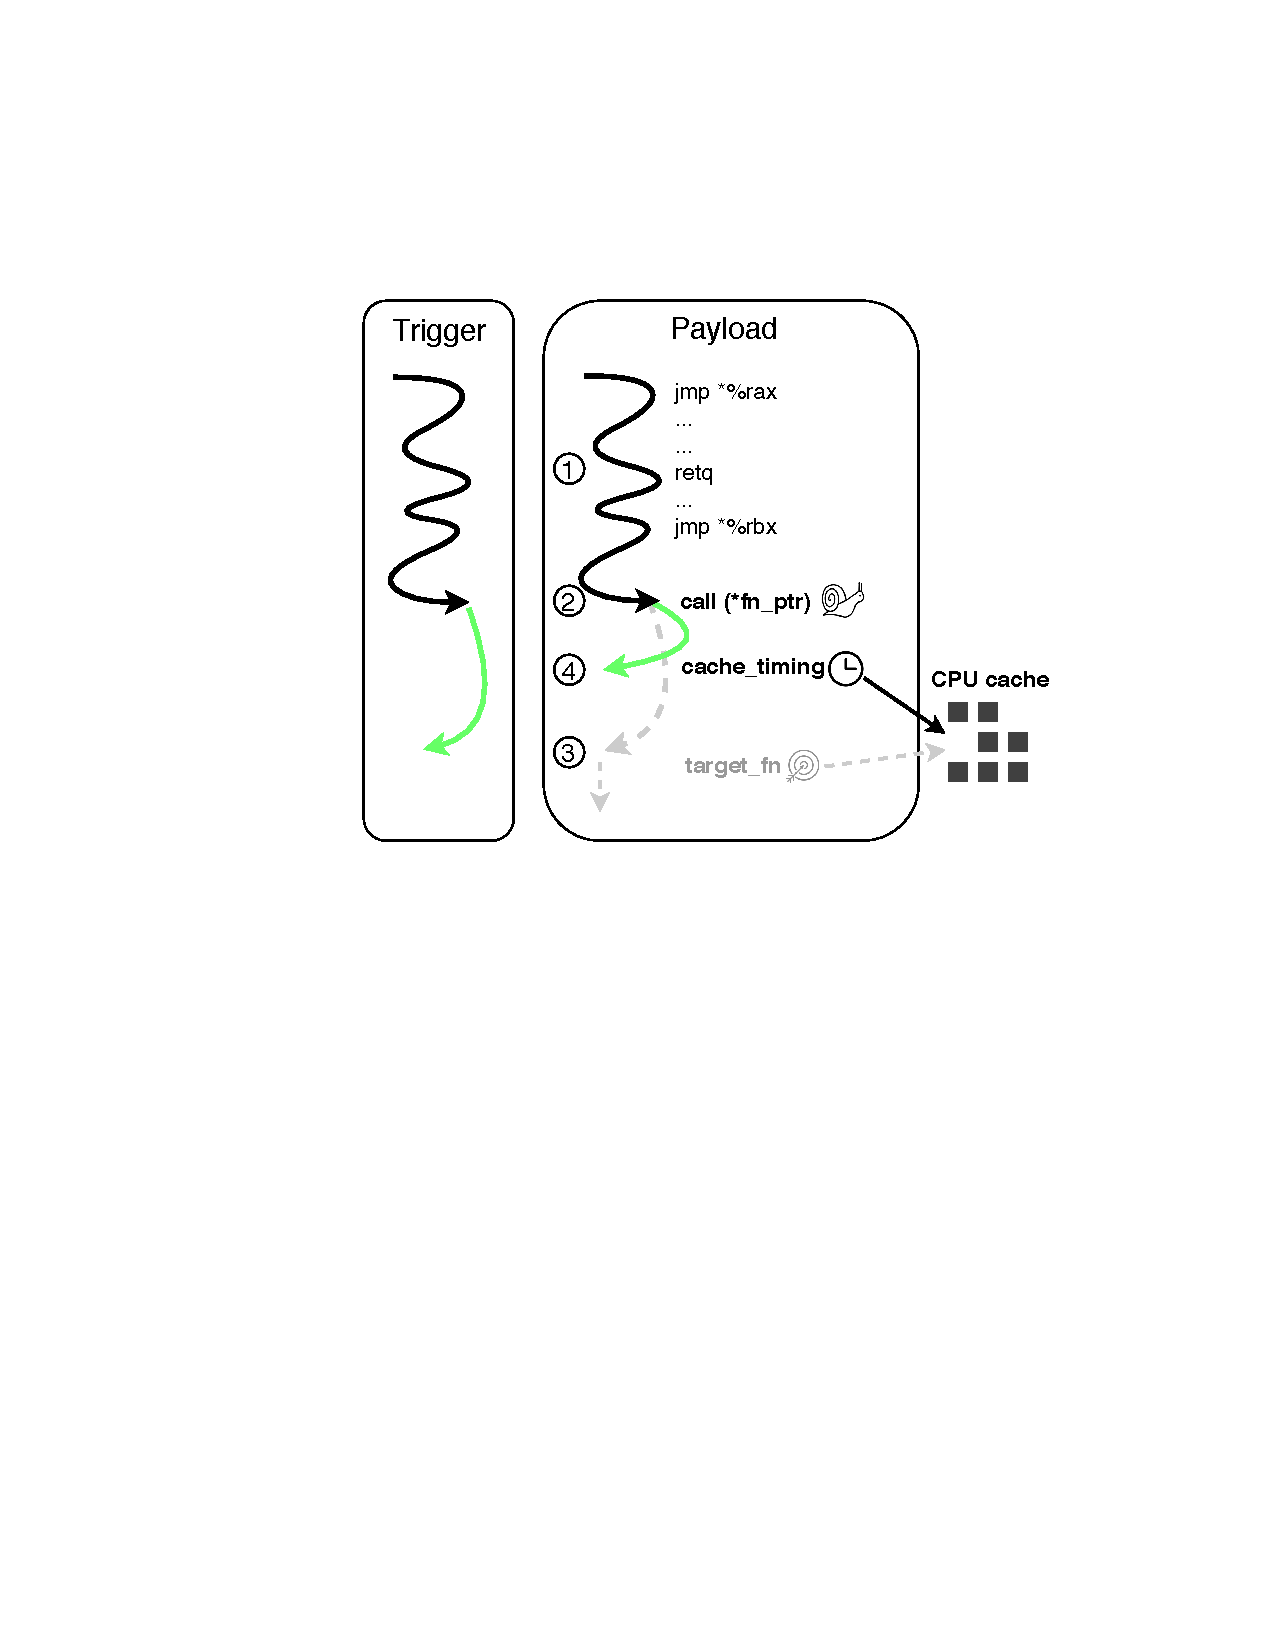
\includegraphics[clip, trim=6cm 13.5cm 3.8cm 5cm, width=0.9\linewidth]{figures/exspectre-high-level.pdf}
    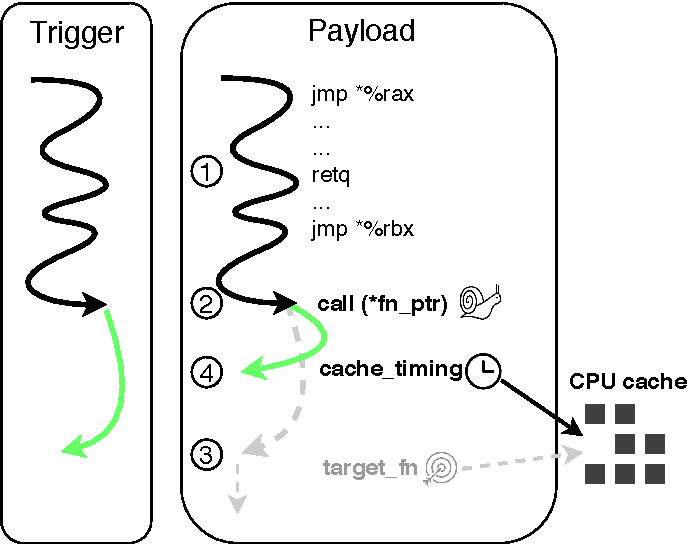
\includegraphics[width=0.9\linewidth]{figures/exspectre-high-level-trimmed.pdf}
    \caption{\textbf{Exspectre}\,---\, %
    1, 2, 3, 4...}

    \label{fig:high-level}

\end{figure}
}


\newcommand{\FigSpecMeasure}{
\begin{figure*}[t]
    \centering
        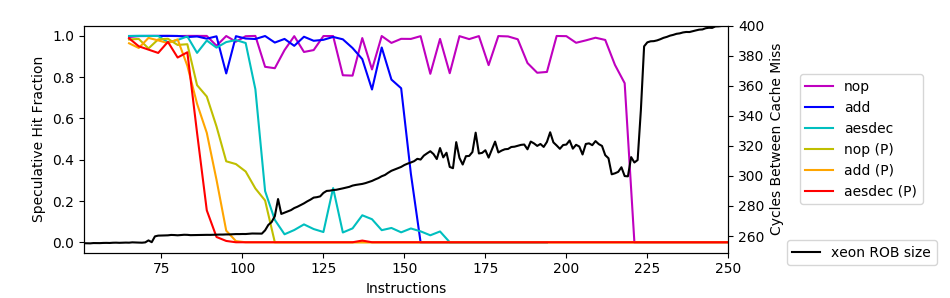
\includegraphics[width=0.9\textwidth]{figures/Speculative_measurements.png}
    \caption{The speculative primitive allows for a limited number of instructions
        to be completed speculatively, dependent on multiple factors. Trigger and 
        payload processes must share cpu resources as they must be performed on 
        the same hyperthread or associated parity hyperthreads. Processes on
        the parity hyperthreads (warm colors) denoted by (P) accomplish a 
        significantly lower number of instructions as compared with processes 
        on the same hyperthread (cool colors).}
    \label{fig:spec-capacity}
\end{figure*}
}


\newcommand{\FigCacheMiss}{
\begin{figure}[h]
    \centering
    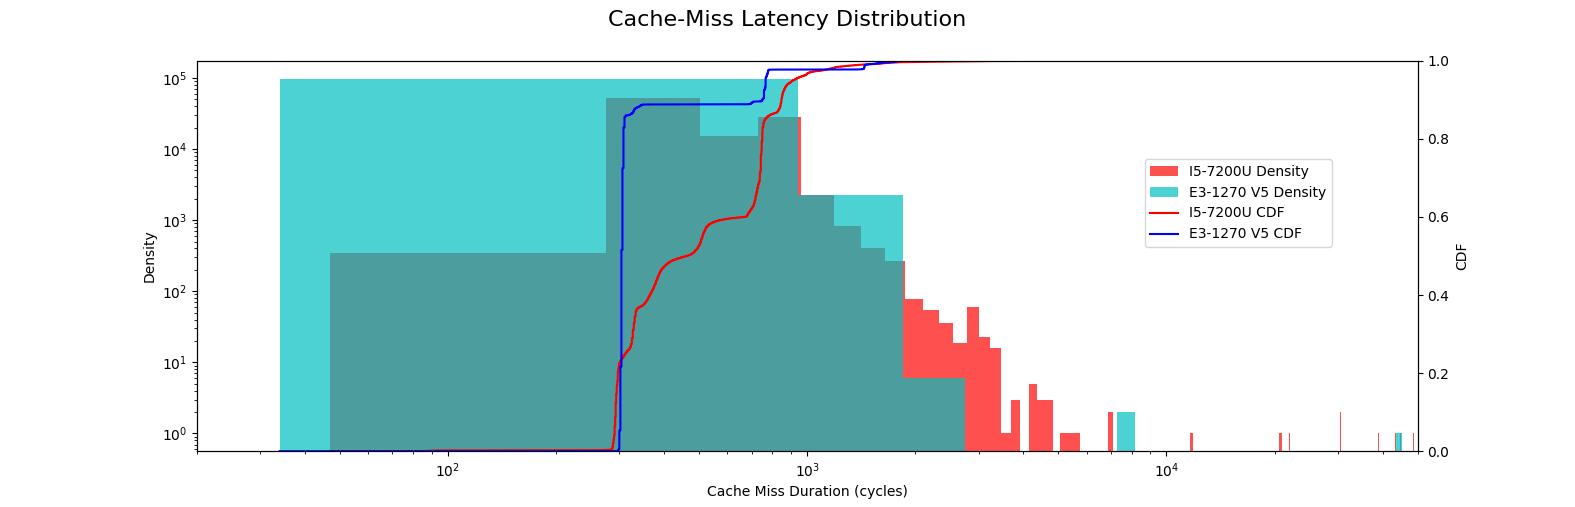
\includegraphics[width=0.5\textwidth]{figures/cache_miss_dist}
    \caption{Cache Hit/Miss Latency Distribution}
    \label{fig:cache-miss}
\end{figure}
}


\newcommand{\FigGeneralModel}{
\begin{figure}[t]
    \centering
        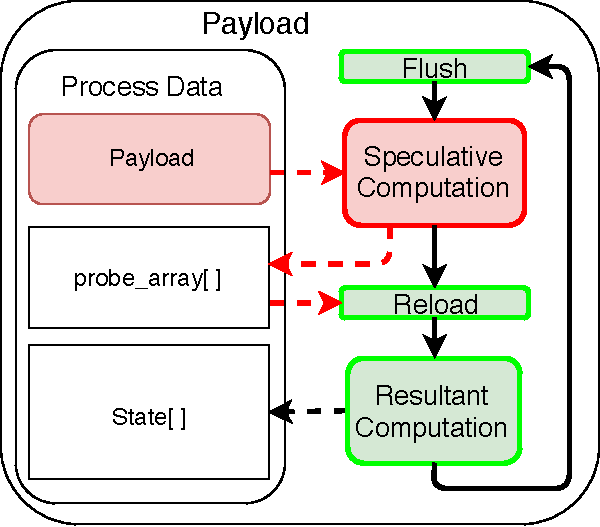
\includegraphics[width=0.4\textwidth]{figures/general_model.pdf}
    \caption{ General model of speculative computation within the Measure 
        process when triggered. \textit{Speculative Computation} has access
        to all variables which do not require a memory transaction within
        the current state of the process. The process can subsequently make
        \textit{Resultant Computations} based on the value returned from 
        \texttt{Flush+Reload} to update the state of the process. }
    \label{fig:general_model}
\end{figure}
}


\newcommand{\FigSpecBandwidth}{
\begin{figure}[t]
    \centering
        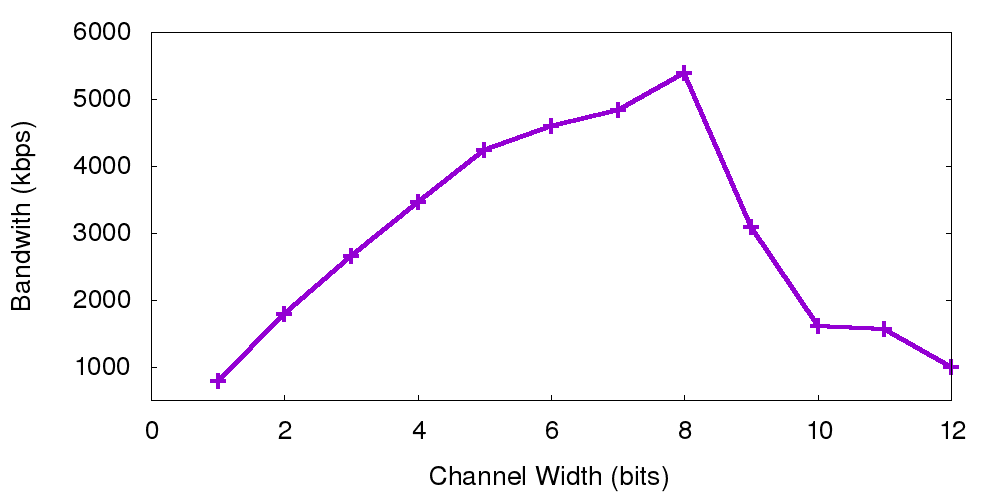
\includegraphics[width=0.5\textwidth]{figures/Speculative_bandwidth}
    \caption{Speculative Bandwidth - Using the speculative primitive 
        1KB of data can be decrypted and exfiltrated at a speed around 5500 kbps
        from the speculative world. Varying the width of the channel 
        results in competing performance factors -- decreasing the 
        number of loops vs decreased size of the probe space.}
    \label{fig:spec_bandwidth}
\end{figure}
}



\newcommand{\FigSpasmModel}{
\begin{figure}[b]
    \centering
        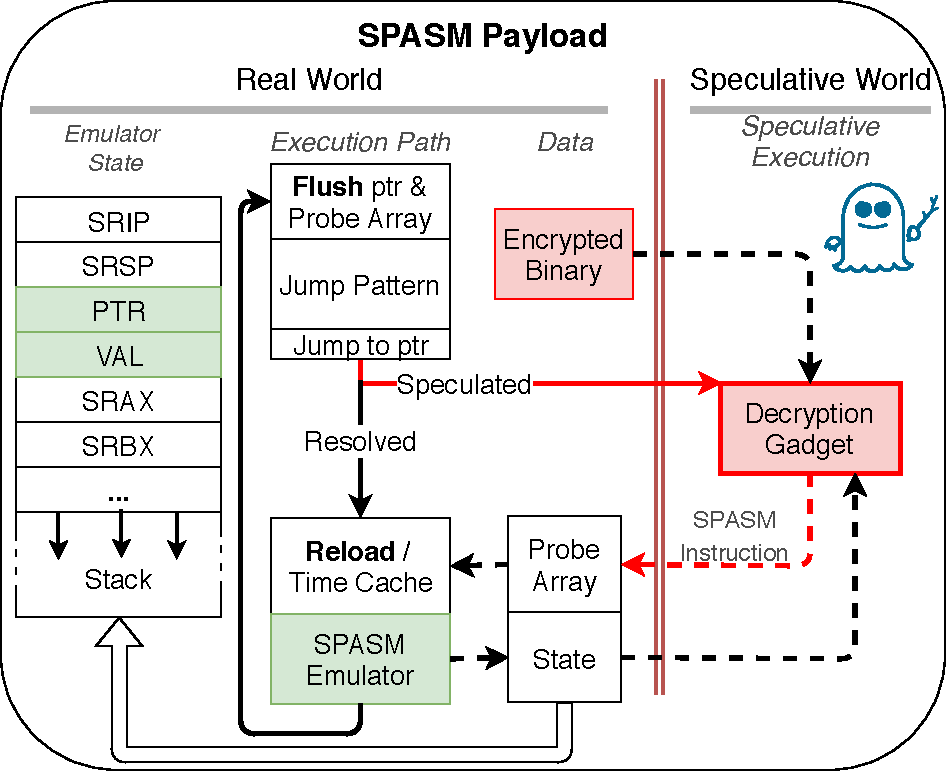
\includegraphics[width=0.5\textwidth]{figures/spasm_model.pdf}
    \caption{This model describes the VM control flow. An encrypted SPASM binary 
        stored in dead code or data accessible to \textit{Speculative Computation} 
        is decrypted  and then returned through the primitive. The SPASM 
        \textit{Resultant Computation} performs the SPASM emulation to update the 
        process state before the next instruction is decrypted.}
    \label{fig:spasm_model}
\end{figure}
}
